\documentclass[12pt]{article}
\setlength{\parindent}{0pt}

\usepackage[utf8]{inputenc}
\usepackage{amsmath}
\usepackage{amsfonts}
\usepackage{amssymb}
\usepackage{amsthm}
\usepackage{graphicx}
\usepackage[labelformat=simple]{subcaption}
\usepackage{verbatim}
\usepackage[left=2.54cm, right=2.54cm, top=2.54cm, bottom=2.54cm]{geometry}
\usepackage{pgf}
\usepackage{tikz,braids}
\usetikzlibrary{positioning}
\usepackage[export]{adjustbox}
\theoremstyle{definition}
\newtheorem{defi}{Definición}[section]
\newtheorem{teor}{Teorema}[section]
\newtheorem{prop}{Proposición}[section]
\newtheorem{ejem}{Ejemplo}[section]
\newtheorem{lema}{Lema}[section]

\renewcommand\thesubfigure{(\alph{subfigure})}
\providecommand{\norm}[1]{\lVert#1\rVert}



\title{Grupo de trenzas y criptografía}
\author{Fernando de la Hoz Moreno}
\date{}
    

\begin{document}

\maketitle

\section{Generalidades sobre grupos}

\begin{defi}[Grupo]
Un grupo es una estructura algebraica formada por un conjundo $G\neq\emptyset$ y una operación interna $G\times G$ a la que llamaremos \textit{producto}. Esta operación asigna a cada pareja $(x,y)$ el elemento $xy$ y verifica las siguientes propiedades:

\begin{enumerate}
\item Propiedad asociativa: $x(yz) = (xy)z$ $\ \ \forall x,y,z\in G$.
\item Existencia de elemento neutro: Existe $1\in G$ tal que $x1= x = 1x\ \ \forall x\in G$.
\item Existencia de elemento simétrico: Para cada $x \in G$ existe $x^{-1}\in G$.
\end{enumerate}
\end{defi}

\begin{prop}
Sea $G\neq\emptyset$ y el producto $G\times G\rightarrow G$ $(x,y)\rightarrow xy$ verificando

\begin{enumerate}
\item Propiedad asociativa: $x(yz) = (xy)z$ $\ \ \forall x,y,z\in G$.
\item Existencia de elemento neutro: Existe $1\in G$ tal que $x1= x = 1x\ \ \forall x\in G$.
\item Existencia de elemento simétrico: Para cada $x \in G$ existe $x^{-1}\in G$.
\end{enumerate}

\end{prop}

\begin{defi}[Subgrupo]
Sea $G$ un grupo. Un subgrupo de $G$ es un subconjunto $H\subseteq G$, $H\neq\emptyset$ que verifica
\begin{enumerate}
\item $xy\in H\ \ \ \forall x,y\in H$ 
\item $1\in H$
\item $x^{-1}\in H\ \ \ \forall x\in H$
\end{enumerate}

Si $H$ es un subgrupo de $G$, lo denotaremos $H\leq G$.



\end{defi}

\begin{defi}[Subgrupo generado]
Sea G un grupo y $X\subseteq G$ un subconjunto $X\neq\emptyset$. Definimos el subgrupo generado por $X$, que denotaremos $<X>$, como el menor subgrupo de $G$ que contiene al conjunto $X$. Se tiene que

$$<X>\ \ =\bigcap_{X\subset K\in Sub(G)}K$$

\end{defi}

\begin{prop}
Para $X\subseteq G$ siendo $X\neq\emptyset$ se tiene que

$$<X>\  = \{x_1^{n_1}x_2^{n_2}\cdot\cdot\cdot x_r^{n_r} :\ x_i\in X,\ n_i\in\mathbb{Z},\ r\geq 1\}$$

\end{prop}

\begin{prop}
Si $G$ es un grupo finito y $X\subseteq G$ siendo $X\neq\emptyset$, entonces

$$<X>\  = \{x_1^{n_1}x_2^{n_2}\cdot\cdot\cdot x_r^{n_r} :\ x_i\in X,\ n_i\in\mathbb{N},\ r\geq 1\}$$

\end{prop}

Denotaremos al subgrupo generado por un único elemento $a\in G$ por $<a>\ = \{a^n:n\in\mathbb{Z}\}$. Si $G$ es finito entonces $<a> = \{a^n:n\geq 0\}$.

Si $X=\{x_1,x_2,...,x_k\}\subseteq G$ es un subconjunto finito entonces $<x_1,x_2,...,x_k>=<X>$.

Si $<X> = G$ diremos que $X$ es un conjunto de generadores de G. Diremos que $G$ es finitamente generado si existe $\{x_1,x_2,...,x_k\}\subseteq G.$ tal que $<x_1,x_2,...,x_k>=G$. Diremos que el grupo G es ciclico si existe $a\in G$ tal que $<a>=G$.



\begin{defi}[Grupo libre]
Sea X un conjunto no vacío. Un par $(F,\kappa:X\rightarrow F)$ donde $F$ es un grupo se dice \textit{universal} para $X$ si para cualquier función $f:X\rightarrow G$ de $X$ al grupo G hay un único homomorfismo de grupo $\tau_f:F\rightarrow G$ tal que

$$\tau_f\circ\kappa = f$$

Al grupo $F$ se le llama \textit{grupo libre} en $X$ y a $X$ se le denomina un conjunto de \textit{generadores libres}.

\end{defi}




\section{El grupo de trenzas de Artin}

Ahora vamos a dar una definición algebraica del grupo de trenzas $B_n$ para cualquier $n>0$. La definición esta formulada en términos de presentación de un grupo por generadores y relaciones.

\begin{defi}
El grupo de trenzas de Artin $B_n$ es el grupo generado por $n-1$ elementos $\sigma_1, \sigma_2,...,\sigma_{n-1}$ y las relaciones de trenza
$$\sigma_i\sigma_j = \sigma_j\sigma_i$$

para todo $i,j=1,2,...,n-1$ con $|i-j|\geq 2$ y

$$\sigma_i\sigma_{i+1}\sigma_i =\sigma_{i+1}\sigma_i\sigma_{i+1}$$

para todo $i=1,2,...,n-2$.
\label{defi:artin}
\end{defi}

\begin{lema}
Si $s_1,...,s_{n-1}$ son elementos de un grupo $G$ que satisfacen las relaciones de trenza, entonces existe un único homomorfismo de grupo $f:B_n\rightarrow G$ tal que $s_i = f(\sigma_i)$ para todo $i=1,2,...,n-1$.
\label{uni_homo}
\end{lema}

\textit{Demostración}. Sea $F_n$ el grupo libre generado por el conjunto $\{\sigma_1,...,\sigma_{n-1}\}$. Hay un único homomorfismo $\bar{f}:F_n\rightarrow G$ tal que $f(\sigma_i)= s_i$ para todo $i=1,...,n-1$. Este homomorfismo induce un homomorfismo de grupo $f:B_n\rightarrow G$ en el que sabemos que si $r$ y $r'$ son dos trenzas tal que $r = r'$ entonces $f(r) = f(r')$. De esta manera obtenemos que el homomorfismo conserva las relaciones de trenza teniendo en cuenta la hipótesis inicial

$$\bar{f}(\sigma_i\sigma_{j})=\bar{f}(\sigma_i)\bar{f}(\sigma_{j})=s_is_j=s_js_i=\bar{f}(\sigma_j)\bar{f}(\sigma_{i})=\bar{f}(\sigma_j\sigma_{i})$$

$$\bar{f}(\sigma_i\sigma_{i+1}\sigma{i}) = s_is_{i+1}s_i=s_{i+1}s_is_{i+1} = \bar{f}(\sigma_{i+1}\sigma_i\sigma_{i+1})$$





\section{Trenzas y sus diagramas}

\begin{comment}
\begin{defi}[$n$-trenza]\label{n_trenza}
Sea $\mathbb{D}$ el cubo unidad, de manera que $\mathbb{D} = \{(x,y,z)\ |\ 0\leq x,y,z\leq 1\}$. En la cara superior del cubo se situan $n$ puntos, $A_1, A_2,...,A_n$, y, de igual manera, se situan $n$ puntos en la cara inferior $B_1, B_2,...,B_n$.
\newline
\newline
Por conveniencia, tomaremos los puntos $A_1=(\frac{1}{2}, \frac{1}{n+1},1),\ A_2=(\frac{1}{2}, \frac{2}{n+1},1),\ ...\ ,\ A_n=(\frac{1}{2}, \frac{n}{n+1},1)$ y $B_1=(\frac{1}{2}, \frac{1}{n+1},0),\ B_2=(\frac{1}{2}, \frac{2}{n+1},0),\ ...\ ,\ B_n=(\frac{1}{2}, \frac{n}{n+1},0)$.
\newline
\newline
Ahora unimos los $n$ puntos $A_1,\ A_2,\ \dotsc\ ,A_n$ con $B_1,\ B_2,\ \dotsc\ ,B_n$ por medio de $n$ segmentos poligonales/arcos $d_1,\ d_2,\ \dotsc\ ,d_n$ (estrictamente hablando, los segmentos deberían ser poligonales, pero, con el fin de hacer los diagramas de manera que sean más faciles de ver al dibujarlos, dibujaremos estos arcos como curvas suaves). Sin embargo, los arcos solo pueden unir de forma que cumplan las siguientes tres condiciones:
\begin{enumerate}
\item $d_1,\ d_2,\ \dotsc\ ,d_n$ son mutuamente disjuntos.
\item Cada $d_i$ conecta algún $A_j$ a algún $B_k$, donde $j$ y $k$ podrían ser o no iguales, pero $d_i$ no permite conectar $A_j$ a $A_k$ (o $B_j$ a $B_k$).
\item Cada plano $E_s$ (llamado plano de nivel), tal que z = s y $s\in [0,1]$ (en otras palabras paralelo al plano-xy) interseca a cada arco $d_i$ en un solo punto.
\end{enumerate}
 Tal configuración de de $n$ arcos $d_1,\ \dotsc\ ,d_n$ (con puntos extremos $A_1,\ A_2,\ \dotsc\ ,A_n$ y $B_1,\ B_2,\ \dotsc\ ,B_n$) es llamada una $n$-trenza, o una trenza con $n$ cadenas. Como cabría de esperar, $d_i$ es llamado una (trenza) cadena (o equivalentemente la $i$-ésima (trenza) cadena).
\end{defi}
\ 
\newline
Vamos a denotar al conjunto de todas las $n$-trenzas por $\mathcal{B}_n$. A continuación definimos un solo movimiento, al que denominaremos como \textit{movimiento elemental}.


\begin{defi}[movimiento elemental]\label{mov_elem}
Supongamos que $\mathbb{D}$ es el cubo unidad y que dentro de este cubo hay un número de cadenas como las definidas en la Definición \ref{n_trenza}. (Para el proposito de esta definición, necesitamos restringir y trabajar exclusivamente con la imagen poligonal de una cadena). Sea $\mathit{AB}$ un segmento de la cadena $d$. Sea $\mathit{C}$ un punto en $\mathbb{D}$ tal que el triángulo $\triangle\mathit{ABC}$ (en $\mathbb{D}$) no interseca a ninguna otra cadena y solo se encuentra con $d$ en $\mathit{AB}$. 
\newline
\newline
Si suponemos que $\mathit{AC}\cup\mathit{CB}$ interseca a todos los planos de nivel $E_s$ con $s\in[0,1]$ como mucho en un punto entonces a la operación de reemplazar $AB$ por $\mathit{AC}\cup\mathit{CB}$, a la cual notaremos por $\Omega$, se le denomina \textit{movimiento elemental}. También podemos realizar la operación inversa, sustituyento $\mathit{AC}\cup\mathit{CB}$ por $AB$, a la que notamos por $\Omega^{-1}$.

\end{defi}

\begin{defi}[Equivalencia de trenzas]\label{eq_trenzas}
Decimos que dos $n$-trenzas, $\beta$ y $\beta'$, son equivalentes si se puede transformar $\beta$ en $\beta '$ tras aplicar un número finito de movimientos elementales sobre $\beta$. Denotamos esta equivalencia como $\beta \sim \beta'$.
\end{defi}

\end{comment}

\begin{defi}[Trenza geométrica]\label{trenza_geom}
Una trenza geométrica de $n$ hebras, con $n \geq 1$, es un subconjunto $\mathcal{B}\subset\mathbb{R}^2\times I$ formado por $n$ intervalos topológicos disjuntos llamados hebras de tal manera que la proyección $\mathbb{R}^2\times I\rightarrow I$ establezca un homeomorfismo de cada hebra en $I$ y
$$$$
$$\mathcal{B}\cap(\mathbb{R}^2\times \{0\})=\{(1,0,0),(2,0,0),...,(n,0,0)\}$$
$$\mathcal{B}\cap(\mathbb{R}^2\times \{1\})=\{(1,0,1),(2,0,1),...,(n,0,1)\}$$
$$$$
Cada hebra de $\mathcal{B}$ interseca con el plano $\mathbb{R}^2\times \{t\}$ con $t\in I$ en un único punto y conecta un punto $(i,0,0)$ con un punto $(s(i),0,0)$ donde $i,s(i)\in\{1,2,...,n\}$. La sucesión $(s(1),s(2),...,s(n))$ es una permutación del conjunto $\{1,2,...,n\}$ llamada permutación subyacente de $\mathcal{B}$
\end{defi}


Decimos que dos trenzas geométricas $\mathcal{B}$ y $\mathcal{B}'$ son isotópicas si podemos deformar de manera continua $\mathcal{B}$ en $\mathcal{B}'$. Más formalmente, $\mathcal{B}$ y $\mathcal{B}'$ son isotópicas si existe una función continua $F : \mathcal{B} \times I \rightarrow \mathbb{R}^2\times I$ de tal manera que para cada $s\in I$, la función $F_s : \mathcal{B}\rightarrow \mathbb{R}^2\times I$ con $F_s(x)= F(x,s)$ es un embebimiento cuya imagen es una trenza geométrica de $n$ hebras, cumpliendo que $F_0 = id_{\mathcal{B}}: \mathcal{B}\rightarrow \mathcal{B}$ y $F_1(\mathcal{B}) = \mathcal{B}'$. Debido a que la imagen de $F_s$ es una trenza geométrica y $F$ es una función continua tenemos automáticamente que la imagen del punto final de cada hebra por $F_s$ es el mismo.
\newline
\newline
Tanto la función $F$ como la familia de hebras geométricas $\{F_s(\mathcal{B})\}_{s\in I}$ se llaman \textit{isotopía} de $\mathcal{B}$ en $\mathcal{B}'$. Se ve facilmente que la relación de isotopía es una relación de equivalencia. Al conjunto de clases de equivalencia correspondientes se les denomina \textit{trenzas de n hebras} y lo denotamos por $\mathcal{B}_n$
\newline
\newline
Para poder especificar una trenza geométrica se puede utilizar la proyección en $\mathbb{R}\times\{0\}\times I$ e indicar de alguna manera que hebra esta por encima de otra cuando se crucen. Solo se podrá aplicar esta solución en trenzas geométricas cuya proyección solo tenga puntos donde se crucen a lo más dos hebras. Pasamos a definir formalmente un diagrama de trenza.


\begin{defi}[Diagrama de trenza]\label{diagrama_trenza}
Un díagrama de trenzas de $n$ hebras es un conjunto $\mathcal{D}\subset\mathbb{R}\times I$ formado por la unión de $n$ intervalos topológicos llamados hebras y que cumplen las siguientes condiciones: 
\begin{enumerate}
\item La proyección de $\mathbb{R}\times I\rightarrow I$ es un homeomorfismo.
\item Cada punto de $\{1,2,...,n\}\times\{0,1\}$ es un punto final de la hebra.
\item Cada punto de $\mathbb{R}\times I$ pertenece como mucho a dos hebras. En cada punto donde se intersequen dos hebras, estas se cruzaran transversalmente.


\end{enumerate}
\end{defi}

La transversalidad de los cruces y la compacidad de las hebras nos asegura que el número de cruces es finito. Gráficamente la hebra que pasa por debajo en un cruce se representará con una discontinuidad y la que pasa por encima con una linea continua. Cada trenza puede ser representada por un diagrama de trenza y cada diagrama tiene asociada una trenza. Dado $\mathcal{D}$ un diagrama, denotaremos como $\beta(\mathcal{D})$ a la trenza de $n$ hebras asociada.
\newline
\newline
Dos diagramas de trenzas $\mathcal{D}, \mathcal{D}'$ de $n$ hebras se dicen que son isotópicos si se puede establecer una función continua entre $F:\mathcal{D}\times I\rightarrow\mathbb{R}\times I$ tal que para cada $s\in I$ el conjunto $\mathcal{D}_s = F(\mathcal{D}\times s)\subset\mathbb{R\times I}$ es un diagrama de $n$ hebras, con $\mathcal{D}_0 = \mathcal{D}$ y $\mathcal{D}_1 = \mathcal{D}'$. Se entiende que $F$ mapea los cruces de $\mathcal{D}$ en los cruces de $\mathcal{D}_s$ para todo $s\in I$ preservando si los cruces son por debajo o por encima. A la familia de diagramas $\{\mathcal{D}_s\}_{s\in I}$ se le llama \textit{isotopía} de $\mathcal{D}_0 = \mathcal{D}$ en $\mathcal{D}_1 = \mathcal{D}'$.




\begin{figure}[h!]
\centering
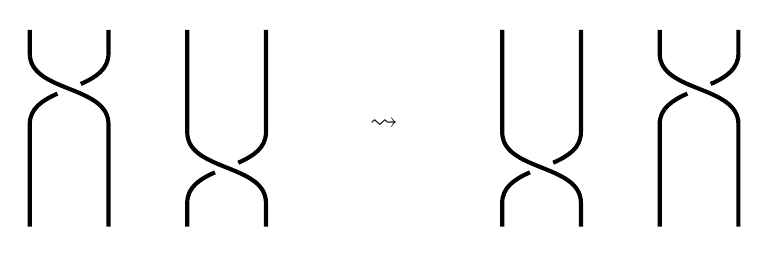
\begin{tikzpicture}
\braid[line width =1.5pt, number of strands = 4, name = b1] (b1) at (-3,0) a_1 a_3;
		\braid[line width =1.5pt, number of strands = 4, name = b1] (b1) at (3,0) a_3 a_1;
		\node[] at (1.5,-1.2){$\leadsto$};
\end{tikzpicture}
\label{fig:d_iso}
\caption{Diagramas isótopicos}
\end{figure}







\begin{defi}[Movimientos de Reidemeister]  Los movimientos de Reidemester  son movimientos locales (afectan a la posición de las hebras dentro de un disco en 
$ \mathbb{R}\times I $ ) en un diagrama de trenzas. Estos estan formados por $\Omega_2$, $\Omega_3$ (Figura \ref{MR}) y sus transformaciones inversas
$\Omega_2^{-1}$, $\Omega_3^{-1}$. 

\end{defi}

\begin{figure}[h!]
\centering
\begin{subfigure}[b]{0.6\linewidth}
\begin{center}
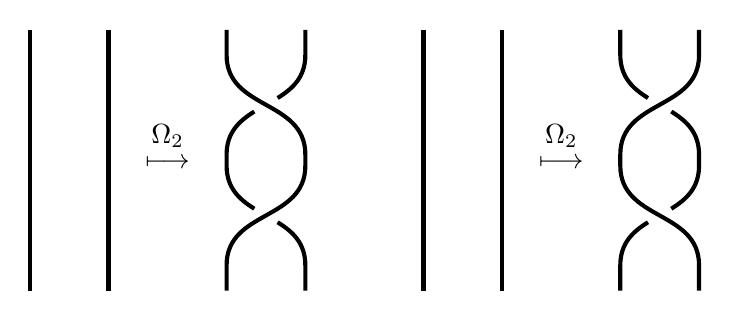
\begin{tikzpicture}
\braid[line width =1.5pt, number of strands = 2, name = b1, height = 80pt] (b1) at (-7,0) a1;
\braid[line width =1.5pt, number of strands = 2, name = b1, height = 40pt] (b1) at (-4.5,0) a_1 a_1^{-1};

		\node[] at (-5.25,-1.7){$\longmapsto$};
		\node[] at (-5.25,-1.35){$\Omega_2$};

\braid[line width =1.5pt, number of strands = 2, name = b1, height = 80pt] (b1) at (-2,0) a1;
\braid[line width =1.5pt, number of strands = 2, name = b1, height = 40pt] (b1) at (0.5,0) a_1^{-1} a_1;

		\node[] at (-0.25,-1.7){$\longmapsto$};
		\node[] at (-0.25,-1.35){$\Omega_2$};
\end{tikzpicture}

\caption{}
\end{center}
\end{subfigure} 


\begin{subfigure}[b]{0.6\linewidth}
\begin{center}
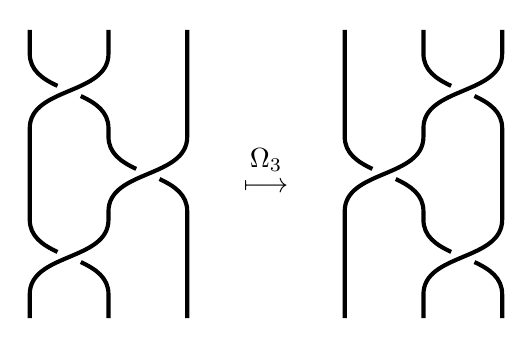
\begin{tikzpicture}
\braid[line width =1.5pt, number of strands = 3, name = b1, height = 30pt] (b1) at (-8.25,0) a_1^{-1}  a_2^{-1} a_1^{-1};
\braid[line width =1.5pt, number of strands = 3, name = b1, height = 30pt] (b1) at (-4.25,0) a_2^{-1} a_1^{-1} a_2^{-1};

		\node[] at (-5.25,-2.0){$\longmapsto$};
		\node[] at (-5.25,-1.65){$\Omega_3$};


\end{tikzpicture}

\caption{}
\end{center}
\end{subfigure} 


\caption{Movimientos de Reidemeister}
\label{MR}
\end{figure}


Estos movimientos preservan la correspondencia entre diagrama de trenza y trenza. Decimos que dos diagramas de trenzas $\mathcal{D}, \mathcal{D}'$ son $\mathcal{R}$\textit{-equivalentes} si $\mathcal{D}$ puede ser transformado en $\mathcal{D}'$ mediante una sucesión finita de isotopías y movimientos de Reidemeister. Esta claro que si $\mathcal{D}, \mathcal{D}'$ son $\mathcal{R}$\textit{-equivalentes}, entonces $\beta(\mathcal{D}) = \beta(\mathcal{D'})$.
\newline

Hemos construido dos equivalencias, una para trenzas geométricas y otra para diagramas de trenzas. El Teorema \ref{teor:equiv} nos permite trabajar indiferentemente con unas o con otras utilizando ambas equivalencias. Tambíen nos garantiza que los diagramas $\mathcal{R}$-\textit{equivalentes} presentan la misma trenza.


\begin{teor}
Dos diagramas de trenzas representan trenzas geométricas isotópicas si y solo si son $\mathcal{R}$\textit{-equivalentes}.
\label{teor:equiv}
\end{teor}
\section{Grupo de trenzas}
\begin{defi}[Producto de hebras]
Dado dos diagrama de trenzas $\mathcal{D}_1$, $\mathcal{D}_2$, representando las trenzas de $n$ hebras $\beta_1$ y $\beta_2$ respectivamente, definimos el producto de diagramas $\mathcal{D}_1\mathcal{D}_2$ concatenando $\mathcal{D}_1$ en la parte superior de $\mathcal{D}_2$ y reduciendo el diagrama resultante en $\mathbb{R}\times I$. Entonces el producto de trenzas $\beta_1\beta_2$ es la trenza  asociada al diagrama producto $\mathcal{D}_1\mathcal{D}_2$.

\end{defi} 

\begin{ejem}
Sean $\beta_1,\beta_2\in \mathcal{B}_3$, cuyos diagramas se pueden ver en \subref{subfig:factores}, el resultado del producto $\beta_1\beta_2$ 
\begin{figure}[h!]
\centering
	\begin{subfigure}[b]{0.45\linewidth}
		\begin{center}
		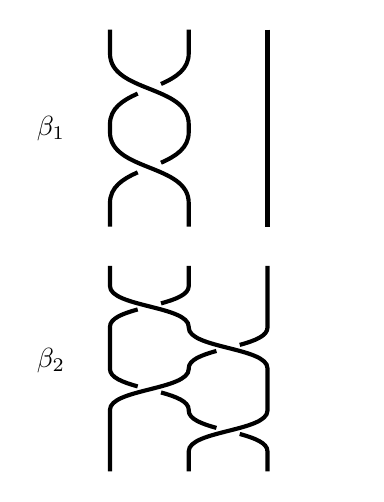
\begin{tikzpicture}
		\braid[line width =1.5pt, number of strands = 3, name = b1] (b1) at (-3,3) a_1 a_1;
	\node[] at (-3.75,1.75){$\beta_1$};
	\node[] at (0,0){};
		\braid[line width =1.5pt, height = 15pt, nudge factor = 0.01, control factor = 0.5, name = b2] (b2) at (-3,0) a_1 a_2 a_1^{-1} a_2^{-1};
		\node[] at (-3.75,-1.2){$\beta_2$};

		\end{tikzpicture}
		\end{center}
		
		\caption{}
		\label{subfig:factores}
	\end{subfigure}
	\begin{subfigure}[b]{0.45\linewidth}
		\begin{center}
		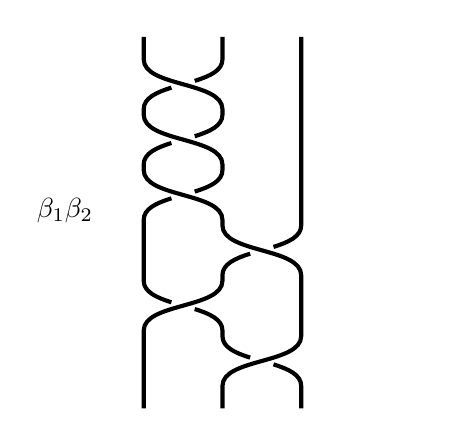
\begin{tikzpicture}
		\braid[line width =1.5pt, height = 20pt, number of strands = 3]  a_1 a_1 a_1 a_2 a_1^{-1} a_2^{-1};
		\node[] at (0,-2.2){$\beta_1\beta_2$};
	\node[] at (4.5,0){};
		\end{tikzpicture}
		\end{center}
		\caption{}
	\end{subfigure}
	\caption{Producto de dos hebras}
	\label{fig:producto_hebras}
\end{figure}
\end{ejem}








\textit{Nota: Formalmente la longitud de los diagramas debería ser constante, pero para una mejor visualización de estos no se ha tenido en cuenta.}
\newline
\newline
De forma clara se ve que el elemento neutro para el producto de trenzas, por ambos lados, es la trenza con el diagrama cuyas hebras se encuentran paralelas entre sí (Figura \ref{fig:elem_neu}).
\begin{comment}
hola
\end{comment}

\begin{figure}[h!]
\begin{center}
		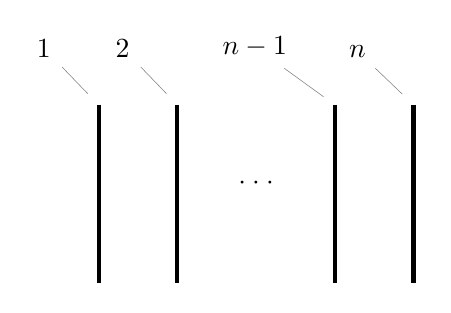
\begin{tikzpicture}
		\braid[line width =1.5pt, height = 50pt, number of strands = 2, name = a]  a1;
		\node[at=(a-1-s),pin=north west:1]  {};
		\node[at=(a-2-s),pin=north west:2]  {};
		\node[] at (3,-1){$\cdot\cdot\cdot$};
		\braid[line width =1.5pt, height = 50pt, number of strands = 2, name = b] at (4,0) a1;
		\node[at=(b-1-s),pin=north west:$n-1$]  {};
		\node[at=(b-2-s),pin=north west:$n$]  {};
		\end{tikzpicture}
		\end{center}
		\caption{Elemento neutro}
		\label{fig:elem_neu}
\end{figure}


Trivialmente también se tiene la asociatividad del producto de trenzas como se puede ver en el ejemplo \ref{ejem:asoci}.

\begin{ejem}[Asociatibidad]





\begin{figure}[h!]
\centering
	\begin{subfigure}[b]{0.8\linewidth}
		\begin{center}
		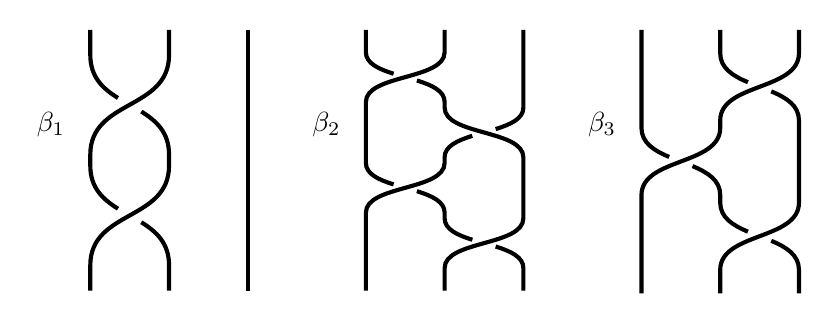
\begin{tikzpicture}
		\braid[line width =1.5pt, number of strands = 3, height = 20pt] (b1) at (-4,0) a_1^{-1} a_2 a_1^{-1} a_2^{-1};
		\braid[line width =1.5pt, number of strands = 3, height = 40pt] (b1) at (-7.5,0) a_1^{-1} a_1^{-1};
		\braid[line width =1.5pt, number of strands = 3, height = 27pt] (b1) at (-0.5,0) a_2^{-1} a_1^{-1} a_2^{-1};
	\node[] at (-4.5,-1.2){$\beta_2$};
	\node[] at (-8,-1.2){$\beta_1$};
	\node[] at (-1,-1.2){$\beta_3$};

		\end{tikzpicture}
		\end{center}
		
		\caption{}
		\label{subfig:factores}
	\end{subfigure}
	
	\begin{subfigure}[b]{0.45\linewidth}
		\begin{center}
		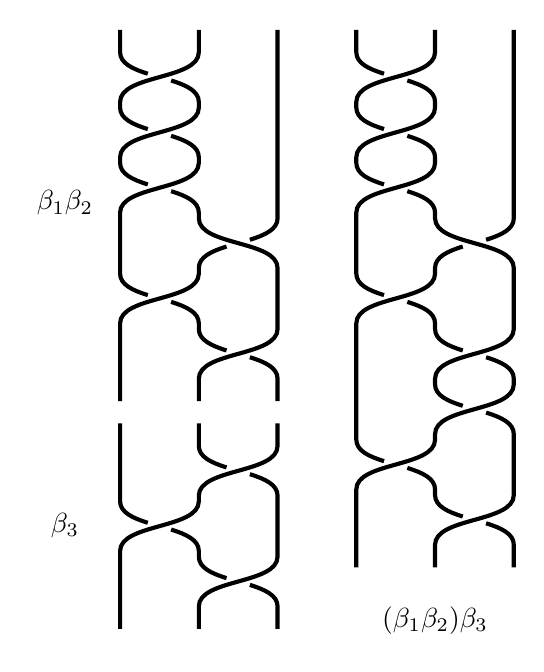
\begin{tikzpicture}
		\braid[line width =1.5pt, height = 20pt, number of strands = 3]  a_1^{-1} a_1^{-1} a_1^{-1} a_2 a_1^{-1} a_2^{-1};
\braid[line width =1.5pt, height = 20pt, number of strands = 3]  at (1,-5) a_2^{-1} a_1^{-1} a_2^{-1};
\braid[line width =1.5pt, height = 20pt, number of strands = 3, height = 20pt] at (4,0) a_1^{-1} a_1^{-1} a_1^{-1} a_2 a_1^{-1} a_2^{-1} a_2^{-1} a_1^{-1} a_2^{-1};
		\node[] at (0.3,-2.2){$\beta_1\beta_2$};

	\node[] at (0.3,-6.3){$\beta_3$};
	\node[] at (5,-7.5){$(\beta_1\beta_2)\beta_3$};
		\end{tikzpicture}
		\end{center}
		\caption{}
	\end{subfigure}
	\begin{subfigure}[b]{0.45\linewidth}
		\begin{center}
		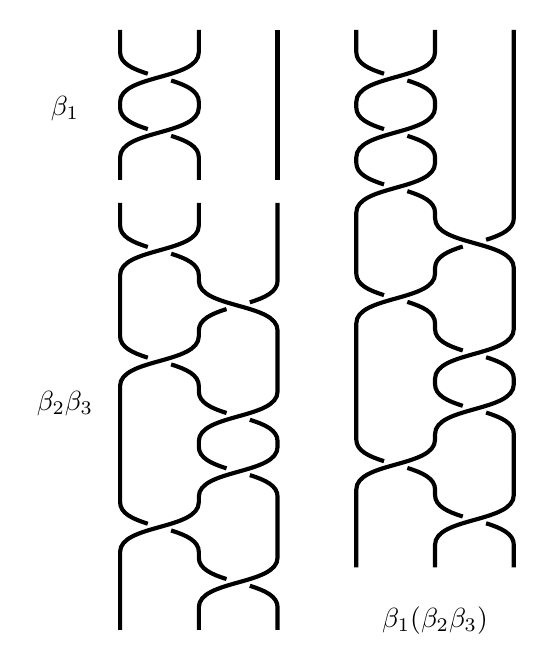
\begin{tikzpicture}
		\braid[line width =1.5pt, height = 20pt, number of strands = 3]  a_1^{-1} a_1^{-1} ;
\braid[line width =1.5pt, height = 20pt, number of strands = 3]  at (1,-2.2) a_1^{-1} a_2 a_1^{-1} a_2^{-1} a_2^{-1} a_1^{-1} a_2^{-1};
\braid[line width =1.5pt, height = 20pt, number of strands = 3, height = 20pt] at (4,0) a_1^{-1} a_1^{-1} a_1^{-1} a_2 a_1^{-1} a_2^{-1} a_2^{-1} a_1^{-1} a_2^{-1};
		\node[] at (0.3,-1){$\beta_1$};

	\node[] at (0.3,-4.75){$\beta_2\beta_3$};
	\node[] at (5,-7.5){$\beta_1(\beta_2\beta_3)$};
		\end{tikzpicture}
		\end{center}
		\caption{}
	\end{subfigure}
	\caption{Asociatividad}
	\label{fig:asoci}
\end{figure}

\label{ejem:asoci}

\end{ejem}

Por último probamos el siguiente lema el cual implica que $\mathcal{B}_n$ es un grupo.

\begin{lema}
\label{lema:inverso}
Sea $\beta\in\mathcal{B}_n$, existe un elemento $\beta^{-1}\in\mathcal{B}_n$ que es el inverso por ambos lados de $\beta$.
\end{lema}
\textit{Demostración}. Para $i = 1,2,n-1$, definimos dos trenzas elementales $\sigma_i^+$ y $\sigma_i^-$ representadas por los diagramas con un unico cruce mostradas en la Figura \ref{fig:elem_braids}. Las trenzas $\sigma_1^+,...,\sigma_{n-1}^+, \sigma_1^-,...,\sigma_{n-1}^-\in\mathcal{B}_n$ generan $\mathcal{B}_n$ como un monoide. Para ver esto, consideramos una trenza $\beta$ de $n$ hebras representada por un diagrama de trenza $\mathcal{D}$. A través de una ligera deformación de $\mathcal{D}\subset\mathbb{R}\times I$ en un vecindario de sus puntos de cruce, podemos hacer que los cruces de $\mathcal{D}$ tengan distinta coordenada. Por tanto podemos establecer una partición

$$0=t_0,t_1,...,t_{k_-1},t_k = 1$$

tal que la intersección de $\mathcal{D}$ con cada banda $\mathbb{R}\times[t_j, t_{j-1}]$ tiene exactamente un cruce dentro. Esta intersección es en realmente un diagrama de $\sigma_i^+$ o $\sigma_i^-$ para algún $i = 1,2,...,n-1$. El resultado de la división de $\mathcal{D}$ como el producto de $k$ diagrama de hebras muestra que

$$\beta = \beta(\mathcal{D}) = \sigma_{i_1}^{\varepsilon_1}\sigma_{i_2}^{\varepsilon_2}\cdot\cdot\cdot\sigma_{i_k}^{\varepsilon_k}$$

donde cada $\varepsilon_j$ es o $+$ o $-$ y $i_1,...,i_k\in{1,2,...,n-1}$.
Claramente, $\sigma_i^+\sigma_i^- = \sigma_i^-\sigma_i^+=1$ para todo $i$. Por tanto $\beta^{-1} = \sigma_{i_k}^{-\varepsilon_k}\cdot\cdot\cdot\sigma_{i_2}^{-\varepsilon_2}\sigma_{i_k}^{-\varepsilon_k}$ (utilizamos el convenio de $--=+\ +-=-$).



\begin{figure}[h!]
\centering
\begin{subfigure}[b]{0.6\linewidth}
\begin{center}
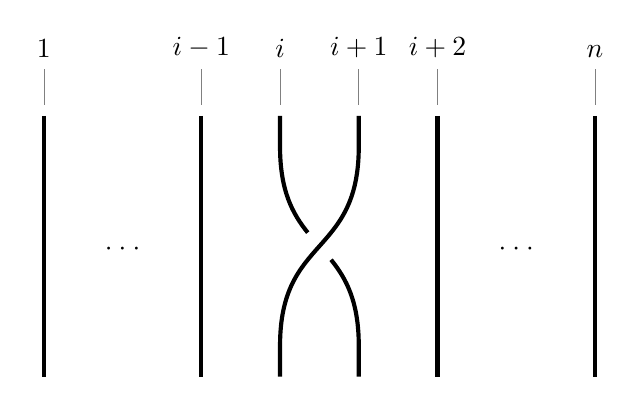
\begin{tikzpicture}
\braid[line width =1.5pt, number of strands = 1, name = a, height = 80pt]  at (-6.75,0) a1;
\braid[line width =1.5pt, number of strands = 4, name = b, height = 80pt] at (-4.75,0) a_2^{-1};
\node[at=(a-1-s),pin=north :1]  {};
\node[at=(b-1-s),pin=north :$i-1$]  {};
\node[at=(b-2-s),pin=north :$i$]  {};
\node[at=(b-3-s),pin=north :$i+1$]  {};
\node[at=(b-4-s),pin=north :$i+2$]  {};

		\node[] at (-5.75,-1.7){$\cdot\cdot\cdot$};



\braid[line width =1.5pt, number of strands = 1, name = c, height = 80pt] at (0.25,0) a1;
\node[at=(c-1-s),pin=north :$n$]  {};

		\node[] at (-0.75,-1.7){$\cdot\cdot\cdot$};

\end{tikzpicture}

\caption*{$\sigma_i^{+}$}
\end{center}
\end{subfigure} 


\begin{subfigure}[b]{0.6\linewidth}
\begin{center}
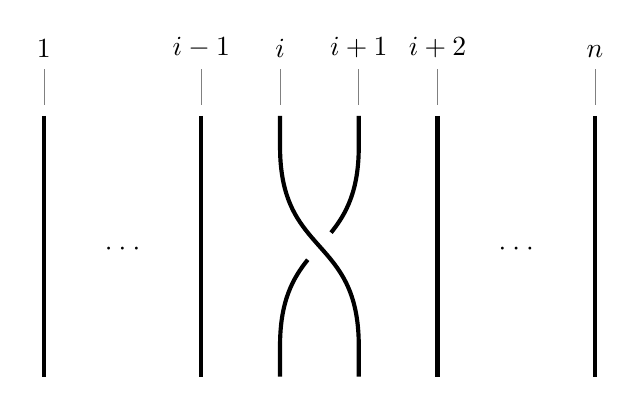
\begin{tikzpicture}
\braid[line width =1.5pt, number of strands = 1, name = a, height = 80pt]  at (-6.75,0) a1;
\braid[line width =1.5pt, number of strands = 4, name = b, height = 80pt] at (-4.75,0) a_2;
\node[at=(a-1-s),pin=north :1]  {};
\node[at=(b-1-s),pin=north :$i-1$]  {};
\node[at=(b-2-s),pin=north :$i$]  {};
\node[at=(b-3-s),pin=north :$i+1$]  {};
\node[at=(b-4-s),pin=north :$i+2$]  {};

		\node[] at (-5.75,-1.7){$\cdot\cdot\cdot$};



\braid[line width =1.5pt, number of strands = 1, name = c, height = 80pt] at (0.25,0) a1;
\node[at=(c-1-s),pin=north :$n$]  {};

		\node[] at (-0.75,-1.7){$\cdot\cdot\cdot$};

\end{tikzpicture}

\caption*{$\sigma_i^-$}
\end{center}
\end{subfigure} 


\caption{Trenzas elementales $\sigma_i^+$ y $\sigma_i^-$}
\label{fig:elem_braids}
\end{figure}

\begin{lema}
Los elementos $\sigma_1^+,...,\sigma_{n-1}^+\in\mathcal{B}_n$ satisfacen las relaciones de trenza, las cuales son, $\sigma_i\sigma_j = \sigma_j\sigma_i$ para todo $i,j=1,2,...,n-1$ con $|i-j|\geq 2$, y $\sigma_i\sigma_{i+1}\sigma_i =\sigma_{i+1}\sigma_i\sigma_{i+1}$ para todo $i=1,2,...,n-2$.
\label{lema:rel_geom}
\end{lema}

\textit{Demostración}. La primera relación viene del hecho de que ambas partes representan diagramas isotópicos. Los diagramas que representan ambos lados de la segunda relación se diferencian por un movimiento de Reidmeister $\Omega_3$.

\begin{teor}
Para $\varepsilon = \pm$, existe un unico homomorfismo $\varphi_\varepsilon : B_n\rightarrow\mathcal{B}_n$ tal que $\varphi_\varepsilon(\sigma_i) = \sigma_i^\varepsilon$ para cada $i=1,2,...,n-1$. El homomorfismo $\varphi_\varepsilon$ es un isomorfismo.
\end{teor}

\textit{Demostración.} Lo probamos para $\varepsilon = +$, el caso $\varepsilon = -$ es quivalente. La existencia y unicidad de $var\phi_+$ vienen proporcionadas por los Lemas \ref{uni_homo} y \ref{lema:rel_geom}. En la prueba del Lema \ref{lema:inverso} se demuestra que $\sigma_1^+,\sigma_2^+,...,\sigma_n^+$ son generadores de $\mathcal{B}_n$. Estos generadores pertenecen a la imagen de $\varphi_+$. Por tanto $\sigma_+$ es sobreyectiva.

Ahora tomamos la función teórica $\psi :\mathcal{B}_n\rightarrow B_n$ tal que $\psi \circ \varphi = id$. Esto implica que $\varphi_+$ es inyectiva. Como en la prueba del Lema \ref{lema:inverso}, representamos cualquier $\beta\in\mathcal{B}_n$ por el diagrama $\mathcal{D}$ en el cual los cruces tienen la segunda coordenada diferente. Esto lleva a una expansión de la forma \label{hola}

\begin{equation}\label{form:expansion}
\psi(\mathcal{D})=(\sigma_{i_1})^{\varepsilon_1}(\sigma_{i_2})^{\varepsilon_2}\cdot\cdot\cdot(\sigma_{i_k})^{\varepsilon_k}\in B_n
\end{equation}

donde $(\sigma_i)^+=\sigma_i$ y $(\sigma_i)^-=\sigma_i^{-1}$. Se tiene que $\psi(\mathcal{D})$ depende exclusivamente de $\beta$. Por el Teorema \ref{teor:equiv} solo nos hace falta verificar que $\psi(\mathcal{D})$ es invariable bajo isotopías y movimientos de Reidmeister sobre $\mathcal{D}$. Isotopías de $\mathcal{D}$ que conservan el orden de los puntos dobles de $\mathcal{D}$ con respecto a la segunda coordenada mantienen la expansión (\ref{form:expansion}) y por tanto preserva $\psi(\mathcal{D})$. Una isotopía que cambia el orden de dos dobles puntos en $\mathcal{D}$ (como en la Figura \ref{fig:d_iso}) reemplaza el termino $\sigma_i^{\varepsilon_i}\sigma_j^{\varepsilon_j}$ en (\ref{form:expansion}) por $\sigma_j^{\varepsilon_j}\sigma_i^{\varepsilon_i}$ para algún $i,j\in\{1,2,...,n-1\}$ con $|i-j|\geq 2$. Bajo $\psi$, a estas expresiones les corresponde el mismo elemento de $B_n$ debido a la primera relación de trenza en Definición
 \ref{defi:artin}.
\newline
\newline
El movimiento $\Omega_2$ (respectivamente $\omega_2^{-1}$) en $\mathcal{D}$ inserta (respectivamente elimina) en la expansion (\ref{form:expansion}) un termino $\sigma_i^+\sigma_i^-$ o $\sigma_i^-\sigma_i^+$. Claramente esto preserva $\psi(\mathcal{D})$.
\newline
\newline
El movimiento $\Omega_3$ en $\mathcal{D}$ reemplaza la secuancia $\sigma_{i}\sigma_{i+1}\sigma_{i}$ en (\ref{form:expansion}) por $\sigma_{i+1}\sigma_{i}\sigma_{i+1}$. Bajo $\psi$, esta expresión corresponde al mismo elemento de $B_n$ debido a la segunda relación de trenza en Definición \ref{defi:artin}. El movimiento $\omega_3^{-1}$ se ve de forma similar.
\newline
\newline

Esto demuestra que $\psi$ es una función bien definida de $\mathcal{B}_n\rightarrow B_n$. Por construcción $\psi\circ\varphi_+=id$. Por tanto $\varphi_+$ es sobreyectiva e inyectiva.




\qed




Sea $\beta\in B_n$ una trenza de $n$ hebras, consideramos una trenza geométrica que la represente . La hebra $d_i$ une el punto $(i,0,0)$ con el punto $(j(i),0,1).$ Definimos la función $\pi:B_n\rightarrow S_n$ del grupo de trenzas al grupo simétrico como

$$\pi(\beta) = \begin{pmatrix}
1 & 2 & \cdot\cdot\cdot & n\\
j(1) & j(2) & \cdot\cdot\cdot & j(n)\\
\end{pmatrix} $$

Da igual la trenza geométrica tomada como representante pueso que todas tienen el mismo punto de inicio y fin para todas las hebras. Podemos decir que $\pi$ es un invariante para las trenzas geométricas y se puede ver facilmente que es un homomorfismo. Normalmente, a la permutación obtenida a partir de una trenza se le denomina \textit{permutación de hebra} y se denota por $\pi(\beta)$.

\begin{defi}[Trenzas puras]
El nucleo del homomorfismo $\pi:B_n\rightarrow S_n$ es llamado \textit{grupo de trenzas puro} y es denotado por $P_n$

$$P_n = Ker(\pi:B_n\rightarrow S_n)$$

Los elementos de $P_n$ se llaman trenzas puras de $n$ hebras. Una trenza geométrica representa a un elemento de $P_n$ si y solo si la hebra que parte de $(i,0,0)$ termina en $(i,0,1)$ 

\end{defi}


\section{Monoides de Garside y Monoides de Trenzas}
Los grupos de trenzas pueden ser vistos como grupos de fracciones de ciertos monoides llamados monoides de trenzas. Estos últimos pertenecen a una clase más amplia de los llamados monoidesde Garside.

\subsection{Monoides}

Un monoide is un conjunto que cuenta con una operación binaria (multiplicación) $M\times M \rightarrow M$ la cual es asociativa y tiene un elemento neutro. Es basicamente un grupo que no cuenta con la propiedad de existencia de elemento simétrico.
\newline
\newline
Un monoide $M$ es \textit{cancelativo por la izquierda} (resp. \textit{por la derecha}) si para todo $a,b,c\in M$

$$ab=ac\Longrightarrow b=c\ \ \ \ (\textrm{resp.}\ \  ba=ca\Longrightarrow b=c)$$
\newline
Un elemento $a$ de un monoide $M$ es \textit{invertible} si existe $b\in M$ tal que $ab=ba=1$.

\subsection{Divisibilidad en monoides}

Si $a=bc$, donde $a,b,c$ son elementos de un monoide $M$, entonces decimos que $b$ es un \textit{divisor por la izquierda} de $a$ y $c$ es un \textit{divisor por la derecha}. También decimos que $a$ es un \textit{múltiplo por la derecha} de $b$ y que $a$ es \textit{múltiplo por la izquierda} de $c$. Lo denotaremos por $b\preceq a$ y $a\succeq c$. Por ejemplo, $1\preceq a$ y $a\succeq 1$ para todo $a\in M$, ya que $a=1a=a1$.

\begin{lema}
Las relaciones $\preceq$ y $\succeq$ en un monoide son reflexivas y transitivas.
\label{lema:rel1}
\end{lema}

\textit{Demostración.} La reflexividad de $\preceq$ viene de la identidad $a=a1$. La transitividad viene dada por la asociatividad de la multiplicacion. Se procede de igual manera para $\succeq$.

\qed


\subsection{Monoides atómicos}

Para cualquier elemento $a\neq 1$ de un monoide $M$, definomos

$$\norm{a}=\sup\{r\geq 1\ | a=a_1\cdot\cdot\cdot a_r,a_1,...,a_r\in M-\{1\}\}$$
\newline
Según esta definición $\norm{a}\in\{1,2,...,\infty\}$. Establecemos que $\norm{1}=0$. Es fácil de ver que para todo $a,b\in M$

$$\norm{ab}\geq\norm{a}+\norm{b}$$
\newline
Observar que$\norm{a}=0$ si y solo si $a=1$. A un elemento $a\in M$ se le llama átomo si $\norm{a}=1$. En otras palabras, $a\in M$ es un átomo si $a\neq 1$ y $a=a_1\cdot\cdot\cdot a_r$ implica que $a_i=1$ para todo $i$ excepto uno. Cualquier $a\in M$ con $\norm{a} < \infty$ tiene una expansión $a=a_1\cdot\cdot\cdot a_r$, donde $\norm{a}=r$ y $a_1,...,a_r$ son átomos. Esto justifica la siguiente definición. Un monoide $M$ es \textit{atómico} si $\norm{a} < \infty$ para todo $a\in M$.

\begin{lema}
Si dos elementos $a,b$ de un monoide atómico $M$ satisfacen $a\preceq b$ y $b\preceq a$, entonces $a=b$.De igual manera, si $a\succeq b$ y $b\succeq a$, entonces $a=b$.
\label{lema:rel2}
\end{lema}
\ 
\newline
\textit{Demostración.} Ya que $a\preceq b\preceq a$, significa que existen $u,v\in M$ tal que $b=au$ y $a=bv$. Entonces $a=auv$ y

$$\norm{a}=\norm{auv}\geq \norm{a}+\norm{u}+\norm{v}$$

Esto implica que $\norm{u}=\norm{v}=0$. Por tanto $u=v=1$ y $a=b$. La relación $\succeq$ es tratada de forma similar.

\qed

Los Lemas \ref{lema:rel1} y \ref{lema:rel2} implican que las relaciones $\preceq$ y $\succeq$ en un monoide atómico son ordenes parciales. Dado un subconjunto $E$ de un monoide atómico $M$, decimos que un elemento $a\in E$ es \textit{maximal} (resp. \textit{minimal}) con respecto a $\preceq$, si $b\preceq a$ (resp. $a\preceq b$) para todo $b\in E$. Un elemento maximal (resp. minimal) de $E$ podría no exisitir, pero si existe, es único por el Lema \ref{lema:rel2}. Definiciones equivalentes se obtienen con la relación $\succeq$.
\newline
\newline
La ecuación $ab=1$ en un monoide atómico $M$ tiene como única solución $a=1,b=1$. De hecho, si $ab=1$ para $a,b\in M$, entonces $1\preceq a \preceq 1$, por lo tanto $a=1$ y $b=1$. En particular, el elemento neutro es el unico elemento invertible de $M$.

\subsection{Presentaciones de un monoide}
Consideramos un conjunto $X$ y un subconjunto $R$ de $X^*\times X^*$. Sea $\sim$ la relación de equivalencia más pequeña conteniendo los pares $(\omega_1r\omega_2, \omega_1r'\omega_2)$, donde $(r,r')\in R$ y $\omega_1,\omega_2\in X^*$. En otras palabras, $\sim$ es la relación de equivalencia más pequeña en $X^*$ tal que $\omega_1r\omega_2\sim\omega_1r'\omega_2$ para todo $(r,r')\in R$ y $\omega_1,\omega_2\in X^*$. Definimos $M$ como el conjunto de clases de equivalencia inducido por $\sim$. Esta claro que $M$ tiene la única estructura de monoide tal que la proyección $P:X^*\rightarrow M$ es un homomorfismo de monoide. Decimos que $\langle X|R\rangle$ es una \textit{presentación de monoide} de $M$ y llamamos a los elementos de $X$ \textit{generadores} y a los elementos de $R$ \textit{relaciones}.
\newline
\newline
Esta claro que el conjunto $P(X)\subset M$ genera $M$ en el sentido de que cada elemento de $M$ es un producto de elementos de este conjunto. Para cada relación $(r,r')\in R$, el elemento $P(r)=P(r')$ de $M$ se le llama \textit{relator} asociado a la presentación $\langle X|R\rangle$. Como notación habitual se usa $r=r'$ para la relación $(r,r'\in R)$ y no se hace distinción entre un generador $x\in X$ y su proyección $P(x)$ en $M$.
\newline
\newline
Introducimos varios tipos de presentaciones de monoides que nos serán de utilidad. Una presentación de monoide $\langle X|R\rangle$ es finita si $X$ y $R$ son finitos. Una presentación $\langle X|R\rangle$ de un monoide $M$ se dice \textit{ponderada} si existe un homomorfismo de monoide $\ell:M\rightarrow \mathbb{N}$ tal que $\ell(x)\geq 1$ para todo $x\in X$. El homomorfismo $\ell$ se llama \textit{peso}.
\newline
\newline
Una presentacion $\langle X|R\rangle$ de un monoide $M$ se dice \textit{equilibrada en longitud} si $l(r)=l(r')$ para todo $(r,r')\in R$, donde $l$ es la función longitud en $X^*$ introducida anteriormente. La formula $\ell(x)=1$ para todo $x\in X$ define un \textit{peso canónico} $\ell:M\rightarrow \mathbb{N}$.

\begin{lema}
Si un monoide $M$ tiene una representación ponderada $\langle X|R\rangle$, entonces $M$ es atómico y todos sus átomos estan contenidos en el conjunto $X$ de generadores. Si $M$ tiene una presentación equilibrada en longitud $\langle X|R\rangle$, entonces el conjunto de átomos de $M$ coincide con $X$ y $\norm{a}=\ell(a)$ para todo $a\in M$, donde $\ell$ es el peso canónico en $M$.
\end{lema}

\textit{Demostración.} Sea $\ell: M\rightarrow \mathbb{N}$ un homomorfismo de monoide tal que $\ell(x)\geq 1$ para todo generador $x\in X$. Entonces $\ell(a)\geq 1$ para todo $a\in M-\{1\}$. Si $a\in M$ se expande como el producto $a_1\cdot\cdot\cdot a_r$ con $a_1,...,a_r\in M-\{1\}$, entonces $\ell(a)=\ell(a_1)+\cdot\cdot\cdot+\ell(a_r)\geq r$. Por tanto $\ell(a)\geq \norm{a}$. Que todos los átomos de $M$ pertenecen a $X$ viene del hecho de que cualquier conjunto que genere un monoide debe contener a sus átomos, ya que estos no se pueden obtener como producto de otros elementos y forman parte del monoide.

\qed

\subsection{El problema de palabra y el problema de divisibilidad}

El \textit{problema de palabra} para una representación $\langle X|R\rangle$ de un monoide $M$ consiste en que dadas dos palabras $\omega,\omega'\in X^*$ representando a los elementos $a,a'\in M$, determinar si $a=a'$. El \textit{problema de dibisibilidad por la izquierda} (resp. \textit{derecha}) esta estrechamente relacionado y consiste en que dadas
dos palabras $\omega,\omega'\in X^*$ representando a los elementos $a,a'\in M$, determinar si $a\preceq a'$ (resp. $a'\succeq a$).
\newline
\newline
Tanto el problema de palabra como el problema de divisibilidad pueden ser facilmente resueltos con una representación finita $\langle X|R\rangle$ de $M$. Sea $\ell:M\rightarrow\mathbb{N}$ un peso, de manera que $\ell(x)\geq 1$ para todo $x\in X$. Observar que el valor de $\ell$ para cualquier $a\in M$ representado por cualquier palabra no vacía $\omega\in X^*$ es mayor o igual que la longitud de $\omega$. Sea $W(a)\subset X^*$
 el conjunto de palabras representando a $a$. Todas esas palabras tienen longitud menor que $\ell(a)$. Ya que $X$ es finito, el número de palabras de menor longitud que $\ell(a)$ es finito y por tanto también lo es el conjunto $W(a)$. Para listar todos los posibles elementos de $W(a)$, uno comienza con la palabra que representa $a$ y consecutivamente aplica todas las posibles subtituciones del tipo
 

$$\omega_1 r\omega_2\leftrightarrow \omega_1 r'\omega_2\ \ \ (r,r')\in R$$

a cualquier elemento de $W(a)$ ya encontrado. Ya que $R$ es finito, este procedidimiento es también finito. Ya que $R$ es finito, este procedimiento también es finito. Esto da una solución al problema de palabra. Dadas dos palabras $\omega,\omega'\in X^*$ representando a $a,a'\in M$ respectivamente, sabemos que $a=a'$ si $W(a)=W(a')$. 
\newline
\newline
También obtenemos una solución para el problema de divisibilidad por la izquierda y por la derecha. Se tiene que $a\preceq a'$ si y solo si algún prefijo (segmento inicial) de una palabra en $W(a')$ pertenece a $W(a)$. De igual manera, $a'\succeq a$ si y solo si algún sufijo (segmento final) de una palabra en $W(a')$ pertenece a $W(a)$

\section{Formas normales y el problema del conjugado}

Ahora vamos a introducir y estudiar un cierto monoide $M_\Sigma$ derivado de un subconjunto $\sigma$ de cierto monoide $M$. Bajo la presunción de hipotesis favorables, obtenemos una forma normal para los elementos de $M_\Sigma$ y resolvemos el problema del conjugado en $M_\Sigma$.

\subsection{El monoide $M_\Sigma$}

Sea $M$ un monoide y $\Sigma\subset M$ un subconjunto de $M$ conteniento el elemento neutro $1$. Sea $M_\Sigma$ un monoide generado por los simbolos $[a]$, donde $a\in \Sigma$, partiendo de la definición de las relaciones $[1]=1$ y $[a][b]=[ab]$, siempre que $a,b,ab\in\Sigma$. Existe un homomorfismo de monoide $p:M_\sigma\rightarrow M$ definido por $p([a])=a$ para todo $a\in\Sigma$.
\newline\newline
Otra definición equivalente de $M_\Sigma$ puede hacerse identificando el producto $[a_1]\cdot\cdot\cdot[a_r]$ en $M_\Sigma$ (donde $a_,...,a_r\in \Sigma$) con la sucesión $(a_1,...,a_r)$. Entonces $M_\Sigma$ es el conjunto de clases de equivalencia de sucesiones finitas $(a_1,...,a_r)$ de elementos de $\Sigma$ bajo la equivalencia generada por

$$(a_1,...,a_{i-1}, a_i'a_i'',a_{i+1},...,a_r)\sim (a_1,...,a_{i-1}, a_i',a_i'',a_{i+1},...,a_r)$$

siempre que $a_i'a_i''\in\Sigma$. La sucesión vacía es equivalente a la sucesión de un elemento $(1)$, donde $1\in\Sigma$. El producto en $M_\Sigma$ esta inducido por la concatenación de sucesiones.





















\section{Introducción a la criptografía}

La \textit{criptografía} es la ciencia de guardar los secretos a salvo. Se asume que un emisor, al que nos referiremos aquí como \textit{Alice}, quiere enviar un mensaje $m$ a un receptor, al que llamaremos \textit{Bob}. Ella usa un canal de comunicación inseguro, como puede ser una red de ordenadores o una linea de teléfono. El problema esta cuando la información que se transmite es confidencial. El mensaje puede ser interceptado y leido o incluso modificado por un agente externo al que nos referiremos como \textit{Eve}. El objetivo de la criptografía es proveer de métodos para evitar este tipo de ataques.

\subsection{Cifrado}

La tarea clásica y fundamental de la criptografía es la de proveer de \textit{confidencialidad} a través de los métodos de cifrado. El mensaje a transmitir se le llama \textit{texto plano}. Alice \textit{cifra} el texto plano $m$ y obtiene un \textit{texto cifrado} $c$. El texto cifrado $c$ es transmitido a Bob. Bob \textit{descifrando} obtiene el texto plano a partir del texto crifrado. Para \textit{descifrar}, Bob necesita una información secreta, la llave de descifrado. La adversaria Eve todavía podría interceptar el mensaje cifrado. Sin embargo, el cifrado del texto plano debería garantizar la confidencialidad y prevenir que pueda extraer alguna información del texto plano a partir del texto cifrado.
\newline
\newline
El cifrado es muy antiguo. Por ejemplo, el \textit{cifrado César} fue introducido hace más de $2000$ años. Cada método de cifrado provee un \textit{algoritmo de cifrado} $E$ y un \textit{algoritmo de descifrado} $D$. En los esquemas de cifrado clásicos, ambos algoritmos dependen de la misma llave secreta $k$. Esta llave $k$ se usa para cifrar y descifrar. A estos métodos de cifrado se les llama \textit{simétricos}.

$$D(k,E(k,m))=m$$

En $1976$, Diffie and Hellman introdujeron el revolucionario concepto de \textit{criptografía de llave pública}. Proporcionaron una solución al problema del intercambio de claves y señalaron el camino a las firmas digitales. A los métodos de \textit{cifrado de llave pública} se les llama \textit{asimétricos}. Cada destinatario de mensajes tiene una llave personal $k = (pk,sk)$ que se compone de dos partes: $pk$ es la lave de cifrado y esta se hace pública, y $sk$ es la llave de descifrado y se mantiene en secreto. Si Alice quiere enviar un mensaje $M$ a Bob, ella cifra $m$ usando la llave de cifrado de Bob $pk$, la cual es pública. Bob descifra el texto cifrado usando su llave de descifrado $sk$ que solo conoce él.

$$D(sk,E(pk,m))=m$$

Cualquiera puede cifrar fácilmente el texto plano usando la llave pública $pk$, pero la otra dirección es complicada. Es practicamente imposible deducir el texto plano a partir del texto cifrado sin saber la llave secreta $sk$.
\newline
\newline
Los métodos de cifrado de llave pública requieren cálculos más complejos y son menos eficientes que los métodos de clásicos de cifrado simétrico. Por eso los métodos simétricos son usados para el cifrado de grandes cantidades de datos. Antes de aplicar el cifrado simétrico, el emisor y el receptor acuerdan una llave. Para mantener la llave en secreto necesitan un canal de comunicación seguro. Lo habitual es utilizar el cifrado de llave pública para este proposito.

\subsection{Objetivos de la criptografía}

Proveer de \textbf{confidencialidad} no es el único objetivo de la criptografía. A su vez esta intenta dar solución a otros problemas. Estos son:

\begin{itemize}
\item \textbf{Integridad de los datos:} El receptor de los datos deberia ser capaz de comprobar si el mensaje ha sido modificado durante la transmisión, ya sea accidentalmente o deliberadamente. Nadie debería ser capaz de alterar total o parcialmente el mensaje original.

\item \textbf{Autenticación:} El receptor del mensaje debería ser capaz de verificar su origen. Nadie debería ser capaz de enviar un mensaje a Bob haciendose pasar por Alice (\textit{autenticación del origen de los datos}). Cuando se inicia la comunicación, Alice y Bob debería ser capaz de identificar el uno al otro (\textit{autenticación de identidad}).

\item \textbf{No repudiación:} El emisor debería no ser capaz negar que envió el mensaje.
\end{itemize}

Hay tanto métodos simétricos como de llave pública para asegurar la integridad de los mensajes. Los métodos simétricos clásicos requieren una llave secreta $k$ que es compartida por el emisor y el receptor. El mensaje $m$ se aumenta con el \textit{código de autenticación de mensaje} (MAC acrónimo en inglés). El código es generado por un algoritmo y depende de una llave secreta. el mensaje aumentado $(m,MAC(k,m))$ está protegido contra modificaciónes. El receptor del mensaje puede comprobar la integridad del mensaje $(m,\overline{m})$ comprobando que

$$MAC(k,m)=\overline{m}$$

Los códigos de autenticación de mensaje se implementan mediante funciones hash con llave.
\newline
\newline
Las \textit{firmas digitales} requieren métodos de llave pública. Como las clásicas firmas a mano, tienen la intención de proveer de autenticación y no repudiación. Las llaves digirales dependen de la clave secreta del firmante (solo pueden ser generadas por él). Por otra parte cualquier persona puede comprobar la validez de la firma utilizando un algoritmo de verificación público \textit{Verify} el cual depende de la llave pública del firmante. Si Alice quiere firmar un mensaje $m$, ella utiliza el algoritmo \textit{Sign} con su llave secreta $sk$ y consigue su firma $Sign(sk,m)$. Bob recibe una firma $s$ para el mensaje $m$ y puede comprobar la firma viendo si

$$Verify(pk,s,m)=ok$$
\ 
con la llave pública de Alice $pk$.
\newline
No es común firmar el mensaje en si mismo, sino usar primero una \textit{función hash criptográfica} y despues firmar el valor hash. Las firmas digitales dependen del mensaje. Mensajes distintos producen firmas distintas. Así que, como los codigos de autenticación de mensaje, las firmas digitales pueden ser utilizadas para garantizar la integridad de los datos.


\subsection{Protocolos criptográficos}

Los algoritmos de cifrado y descifrado, funciones hash criptográficas y los generadores peusoaleatorios son básicamente los bloques de construcción (también llamados primitivas criptográficas) utilizados para resolver problemas que involucran confidencialidad, autenticación o integridad de los datos.
\newline
\newline
En muchos casos un único bloque de construcción no puede resolver un problema, sino que se necesita combinar varias primitivas. Una serie de pasos deben ser ejecutados para completar la tarea. A la sucesión de pasos bien definidos se le denomina \textit{protocolo criptográfico}. Es habitual añadir una condición a esta definición y es la de dos o más partes esten involucradas. Solo usaremos el término ``protocolo'' si se requiere al menos dos personas para completar la tarea.
\newline
\newline
Como contraejemplo echamos un vistazo al esquema de firma digital. Un esquema típico para generar una firma digital es primero aplicar una función hash criptográfica $h$ al mensaje $m$ y después, en un segundo paso, calcular la firma utilizando el algoritmo de descifrado de llave pública sobre el valor hash $h(m)$. Ambos pasos estan hechos por una única persona, por lo que no se considera un protocolo.

\subsubsection{Intercambio de llaves}
Los criptosistemas de llave pública y secreta asumen que los participantes tienen acesso a las llaves. En la práctica, uno puede utilizar estos sistemas si el problema de la distribución de llaves esta resuelto.

El concepto de seguridad para llaves tiene dos niveles. El primer nivel emplea llaves secretas de larga duración, denominadas \textit{llaves maestras}. Las llaves del segundo nivel estan asociadas con la sesión, por lo que son llamadas \textit{llaves de sesión}. Una llave de sesión es solo válida durante el breve tiempo de duración de una sesión. Las llaves maestras son normalmente las llaves empleadas en un criptosistema de llave pública.
\newline
\newline
Hay dos razones principales para el concepto a dos niveles. La primera es que el cifrado por llave simétrica es más eficiente que el cifrado de llave pública. por tanto, las llaves de sesión suelen ser llaves de criptosistemas simétricos, y esas deben ser intercambiadas de manera segura, usando otras llaves. La segunda razón y probablemente más importante es que el concepto a dos niveles provee de más seguridad. Si la seguridad de una sesión se ve comprometida, solo afecta a esa sesión. Dada una llave de sesión, el número de textos cifrados disponibles para el criptoanalisis es limitado. Las llaves de sesión son generadas cuando se necesitan utilizar y se desechan después de ser usadas.
\newline
\newline
La llave maestra se utiliza para generar las llaves de sesión. Por tanto es especialmente importante prevenir los ataques sobre la llave maestra. Por eso el acceso a la llave maestra esta estrictamente limitado.





















\section{Plataformas criptograficas y grupos de plataforma}

Si un protocolo criptográfico esta basado en un objeto algebraico como puede ser un grupo, un anillo u otros, entonces es llamado \textit{plataforma criptográfica} o \textit{plataforma}. En criptografía basada en un grupo a este se le llama \textit{grupo de plataforma} para el protocolo criptográfico. La seguridad de un protocolo criptográfico depende entonces de la dificultad, computacional o teórica, de resolver un problema de teoría de grupos en el grupo de plataforma.
\newline
\newline
Para que un grupo de plataforma $G$ sea adecuado para un protocolo criptográfico basado en grupos, $G$ debe poseer ciertas propiedades que hagan el protocolo tanto eficiente de implementar como seguro. Se asume que el grupo posee una representación finita

$$G = \langle X;R\rangle=\langle x_1,...,x_n: R_1=\cdot\cdot\cdot=R_m=1\rangle$$

y que el protocolo de seguridad esta basado en un problema de teoría de grupos que denotamos por $\mathcal{P}$. La primera necesidad es que haya una forma de representar unicamente y multiplicar los elementos de $G$. En la mayoría de casos esto requiere una \textit{forma normal} para los elementos $g\in G$ en término de unos generadores $\{x_1,...,x_n\}$. Una forma normal es, para cada $g\in G$, una única representación en término de los generadores. Las formas normales proveen de un método efectivo para distinguir los elementos del grupo. La existencia de una forma normal en un grupo implica que el problema de palabra tiene solución para este, lo que es esencial para estos protocolos. Para $g\in G$ denotaremos su forma normal, en términos del conjunto de generadores $X$, por $NF_X(g)$. Para que sea útil en criptografía, dado $g\in G$ expresado como una palabra en $x_1,...,x_n$, el proceso de pasar de la palabra a la forma normal única debe ser computacionalmente eficiente.
\newline
\newline
Además de que el grupo de plataforma tenga forma normal, idealmente debería presentar un crecimiento exponencial. Es decir, que la función crecimiento para $G$,

$$\gamma:\mathbb{N}\rightarrow\mathbb{R}$$
$$\gamma(n)=\#\{w\in G:l(w)\leq n\}$$

tiene un ratio de crecimiento exponencial. En la definición $l(w)$ se entiende como el número de letras mínimo necesitado para expresar $w$ como una palabra en $x_1,...,x_n$. El crecimiento exponencial es necesario, ya que esto asegura tener un gran espacio de llaves, haciendo que una búsqueda de fuerza bruta para la llave secreta sea un algoritmo no factible.
\newline
\newline
A parte la forma normal debe presentar buena difusión al determinar las formas normales de los productos. Esto quiere decir que al encontrar la forma normal de un producto es difícil computacionalmente descubrir los factores. Esto es formalmente que si nosotros conocemos $NF_X(g_1g_2)$ es difícil computacionalmente encontrar $g_1,g_2$ o $NF_X(g_1)$,$NF_X(g_2)$
\newline
\newline
Otras necesidades para el grupo plataforma dependen del protocolo en particular. Si la seguridad esta basada en el problema de grupo $\mathcal{P}$, tales como el problema de palabra o el problema del conjugado, se tiene que asumir que en $G$, la solución a $\mathcal{P}$ es computacionalmente compleja (NP-Complejo) o irresoluble. Sin embargo, lo que realmente queremos es que sea \textit{generalmente complejo}, es decir, complejo para la mayoría de entradas. La solución de $\mathcal{P}$ podría ser irresoluble pero tener una complejidad en el caso promedio polinomial. En este caso, si no tenemos cuidado al elegir las entradas, la solución de $\mathcal{P}$ es fácil y el protocolo criptográfico esta roto. Esto no elimina a $G$ como un posible grupo de plataforma pero indica que hay que tener cuidado al escoger las entradas.

Entre los primeros intentos de usar grupos no abelianos como plataformas para criptosistemas de llave pública estuvieron los esquemas de Anshel-Anshel-Goldfeld y Ko, Lee et al. 

\section{Los protocolos Ko-Lee y Anshel-Anshel-Goldfeld}

Todos los protocolos basados en grupos no abelianos dependen de la dificultad de resolver ciertos problemas de decisión de grupo y problemas computacionales de teoría de grupos. Recordar que el \textit{problema del conjugado}, también llamado \textit{problema de decisión del conjugado}, para un grupo $G$, o más precisamente para una presentación de grupo es el que sigue: dados $g,h\in G$, determinar algoritmicamente si son conjugados, es decir, si existe $z\in G$ tal que $g = zhz^{-1}$. El problema del conjugado es irresoluble en general, lo que quiere decir que existen presentaciones de grupos para los cuales no existe un algoritmo que resuelva el problema del conjugado. Por ejemplo, el problema del conjugado es resoluble para grupos libres y grupos hiperbólicos libres de torsión.
\newline
\newline
Lo relevante para el protocolo Ko-Lee es el \textit{problema de búsqueda del conjugador}. Este consiste en que, dado una presentación de grupo para G, y dos elementos $g_1,g_2\in G$, los cuales se saben que son conjugados determinar algoritmicamente un conjugador, es decir, un elemento $h\in G$ tal que $g_1 = hg_2h^{-1}$. El problema de búsqueda del conjugador es en general indecidible en general, como el problema del conjugado.

\subsection{Protocolo Ko-Lee}
Ko, Lee et al desarrollaron un sistema de intercambio de llave pública que es una traducción  directa del protocolo Diffie-Hellman a una configuración de teoría de grupos no abelianos. Su seguridad esta basada en la dificultad del problema del conjugado. 
\newline
\newline
En cualquier grupo de platadorma $G$ dados dos elementos $g,h\in G$ denotaremos el conjugado de $g$ por $h$ como $g^h$, tal que $g^h = hgh^{-1}$. Facilmente se comprueba que dados $g,h_1,h_2$ entonces $(g^{h_1})^{h_2}=g^{h_1h_2}$.

$$(g^{h_1})^{h_2}= h_2^{-1}g^{h_1}h_2= h_2^{-1}h_1^{-1}gh_1h_2 = (h_1h_2)^{-1}g(h_1h_2) =g^{h_1h_2}$$

Tomamos un grupo de plataforma $G$ que posee todas las propiedades deseables anteriormente mencionadas. Además asumimos que $G$ tiene una colección grande de subgrupos (no cíclicos) tal que conmutan los elementos entre sí. Esto quiere decir que si tomamos $A,B$ dos de estos subgrupos y $a\in A, b \in B$ entonces $ab=ba$.

Alice y Bob escogen un par de estos subgrupos del grupo de plataforma $G$. $A$ es el subgrupo de Alice y $B$ es el subgrupo de Bob y estos son secretos



\section{Esquemas criptográficos basados en trenzas}

\subsection{Intercambio de llaves}
Alice y Bob desean compartir una llave secreta, de tal manera que un intruso que esté observando la comunicación no pueda deducir ninguna información útil sobre un secreto en común.
\subsubsection{Esquema Anshel-Anshel-Goldfeld}
Propuesto por Anshel \& al. este esquema es una plataforma criptográfica en el que se puede utilizar cualquier grupo de plataforma en el que el Problema de Búsqueda del Conjugado sea lo suficientemente complicado.

La llave pública consiste en dos conjuntos de trenzas $\{p_1,...,p_l\},\{q_1,...,q_m\}\subset B_n$. La llave secreta de Alice es una palabra $u$ formada por $l$ letras y sus inversas y la llave secreta de Bob es una palabra $u$ formada por $m$ letras y sus inversas. El intercambio de llave esta esta compuesto de los siguientes pasos:

\begin{enumerate}
\item Alice calcula la trenza $s = u(p_1,...,p_l)$ y lo usa para calcular los conjugados $q_1'=sq_1s^{-1},...,q_m'=sq_ms^{-1}$. Ella envía $q_1',...,q_m'.$
\item Bob calcula la trenza $r = v(q_1,...,q_m)$ y lo usa para calcular los conjugados $p_1'=sp_1s^{-1},...,p_l'=sp_ls^{-1}$. Ella envía $p_1',...,p_l'.$
\item Alice calcula $t_A = su(p_1',...,p_l')^{-1}$
\item Bob calcula $t_B = v(q_1',...,q_m')r^{-1}$
\end{enumerate}

La llave compartida es $t_A = t_B$. Sabiendo que 
$$u(p_1',...,p_l')=r\ u(p_1,...,p_l)r^{-1}$$
$$v(q_1',...,q_m')=s\ v(q_1,...,q_m)s^{-1}$$
Es fácil ver que

$$t_A = s\ u(p_1',...,p_l')^{-1} = s\ r\ u(p_1,...,p_l)^{-1}r^{-1}=$$
$$=s\ r\ s^{-1}r^{-1}= s\ v(q_1,...,q_m)\ s^{-1}r^{-1}=v(q_1',...,q_m')r^{-1} = t_B$$

La seguridad esta basada en la dificultad de resolver una variante del Problema de Búsqueda del Conjugado en $B_n$, que es llamado el Problema de Búsqueda del conjugado Múltiple, en el cual se intenta encontrar una trenza conjugadora no de un único par de trenzas conjugadas $(p,p)$ sino de una familia finita de pares de trenzas $(p_1,p_1'),...,(p_l,p_l')$. Nótese que el Problema de Búsqueda del Conjugado Múltiple es más facil que el Problema de Búsqueda del Conjugado, puesto que se tiene más información de los conjugadores. Sin embargo, es lo suficientemente complejo como para que el intruso sea incapaz de encontrar la llave secreta $r$ conociendo los pares $(p_1,p_1'),...,(p_l,p_l')$. De igual manera, no será capaz de encontrar la llave secreta $s$ conociendo los pares $(q_1,q_1'),...,(q_m,q_m')$.

\subsubsection{Esquema Diffie-Hellman} Aunque los grupos de trenzas no son conmutativos, estos contienen grandes subgrupos donde para cada elemento de un primer subgrupo conmutan con cada elemento de un segundo subgrupo. De hecho, las trenzas que involucran conjuntos distintos de hebras conmutan. Si denotamos por $LB_n$ (respectivamente $UB_n$) al subgrupo de $B_n$ generado por $\sigma_1,...,\sigma_{m-1}$ (respectivamente $\sigma_{m+1},...,\sigma_{n-1}$) con $m=[n/2]$, cada trenza en $LB_n$ conmuta con cada trenza en $UB_n$.

Esta observación es utilizada por el esquema de intercambio de llave Diffie-Hellman propuesto por Ko \& al. En este, la llave pública consiste en una trenza $p$ en $B_n$. La llave secreta de Alice es una trenza $s$ en $LB_n$. La llave secreta de Bob es una trenza $r$ en $UB_n$. El intercambio esta formado por los siguientes pasos:

\begin{enumerate}
\item Alice calcula el conjugado $p'=sps^{-1}$, y se lo envia a Bob.
\item Bob calcula el conjugado $p''=rpr^{-1}$, y se lo envia a Alice.
\item Alice calcula $t_A = sp''s^{-1}$.
\item Bob calcula $t_B = rp'r^{-1}$. 
\end{enumerate}

La llave compartida es $t_A = t_B$. Esto es debido a que $s$ y $r$ conmutan:

$$t_A=s\ p''s^{-1}=s\ r\ p\ r^{-1}s^{-1} = r\ s\ p\ s^{-1}r^{-1} = r\ p'r^{-1}=t_B$$

Aquí la seguridad también esta basada en la dificultad de resolver una variante del Problema de Búsqueda del Conjugado donde dada una trenza $p$ de $B_n$ y las trenzas $p'=sps^{-1}$ y $p''=rpr^{-1}$, con $s$ y $r$ pertenecientes a $LB_n$ y $UB_n$ respectivamente, hay que encontrar la trenza $rp'r^{-1}$ o lo que es igual $sp''s^{-1}$. El problema es lo bastante complejo como para no poder encontrar $rp'r^{-1}=sp''s^{-1}$ conociendo los pares $(p,p')$ y $(p,p'')$

\subsection{Cifrado}
Aquí el problema es que Bob desea enviar un mensaje $m$ a Alice, y el puede usar la llave pública de Alice para cifrar su mensaje. Alice debe ser capaz de recuperar el mensaje original de Bob usando su llave privada, de manera que un intruso que observe la comunicación no pueda.

\subsubsection{Esquema Ko \& al.}
La notación será la empleada en el esquema de intercambio de llaves previo. Además, asumimos que $h$ es una \textit{función hash unidireccional libre de colisión} de $B_n$ a $\{0,1\}^N$, es decir, una función calculable tal que la probabilidad de que $h(b_1)=h(b_2)$ para $b_1\neq b_2$ es despreciable (libre de colisión) y recuperar $b$ a partir de $h(b)$ es inviable.
\newline
\newline
Comenzamos con $p\in B_n$ y $s\in LB_n$. La llave pública de Alice es el par $(p,p')$, con $p'=sps^{-1}$. La llave privada de Alice es $s$. Con el fin de enviar el mensaje $m_B$, el cual asumimos que se encuentra en $\{0,1\}^N$, usando $\oplus$ para la operación Booleana ``or-exclusivo"(es decir, la suma en $\mathbb{Z}/2\mathbb{Z}$):

\begin{enumerate}
\item Bob elige una trenza aleatoria $r$ en $UB_n$ y envia el texto cifrado $m''=m_B\oplus h(rp'r^{-1})$ junto con el dato auxiliar $p''=rpr^{-1}$.
\item Alice calcula $m_A = m_B$. 

\end{enumerate}

Entonces tenemos que $m_A = m_B$ es decir, Alice recupera el mensaje original de Bob. Esto se debe a que las trenzas $r$ y $s$ conmutan

$$sp''s^{-1}=s\ r\ p\ r^{-1}s^{-1}=r\ s\ p\ s^{-1}r^{-1}$$

y entonces tenemos que 

$$m_A = m_B\oplus h(rp'r^{-1})\oplus h(sp''s^{-1})=m_B$$

Aquí la seguridad esta basada en la dificultad del Problema del Conjugado inspirado en Diffie-Hellman para $B_n$. Bajo las hipótesis sobre $h$, ser capaz de romper el sistema implica tener que recuperar los valores comunes $rp'r^{-1}$ y $sp''s^{-1}$ a partir de los pares $(p,p')$ y $(p,p'')$.

\subsection{Autenticación de identidad}
Ahora el problema es que Alice desea probar su identidad a Bob, es decir, ella desea probar que conoce la llave privada sin permitir que un intruso que observe la comunicación deduzca nada sobre su llave privada.

\subsubsection{Esquema inspirado en Diffie-Hellman}. El siguiente esquema desafío-respuesta esta ínspirado en el esquema previo de Ko \& al. La llave pública es un par de trenzas conjugadas $(p,p')$ en $B_n$ con $p'=sps^{-1}$, mientras que la llave privada de Alice es la trenza $s$ utilizada para conjugar $p$ y $p'$. Asumimos que $s\in LB_n$. También usaremos $h$ como función hash unidireccional libre de colisión en $B_n$. Entonces para realizar la autenticación se hace el siguiente intercambio:

\begin{enumerate}
\item Bob elige una trenza aleatoria $r\in UB_n$, y le envía el desafío $p''=rpr^{-1}$ a Alice.
\item Alice le envía la respuesta $y = h(sp''s^{-1})$.
\item Bob comprueba que $y=h(rp'r^{-1})$
\end{enumerate}

Una respuesta correcta por parte de Alice implica la aceptación por parte de Bob, debido a que las trenzas $r$ y $s$ conmutan, y por tanto, tenemos que $rp'r^{-1}=sp''s^{-1}$. Por otra parte, la aceptación ocurre solo si la respuesta de $y$ de $A$ satisface $y=h(rp'r^{-1})$, por tanto, bajo las hipotesis de $h$, solo si Alice ha sido capaz de resolver el Problema del Conjugado inspirado en Diffie-Helman para $B_n$. Una vez más, la seguridad recae en la dificultad de resolver este problema.


\subsubsection{Esquema inspirado en Fiat-Shamir} Este esquema de autenticación es propuesto por Sibert \& al. Este esquema hereda del esquema Fiat-Shamir lo que implica repetir varias el desafío-respuesta en tres pasos. Como antes, las llaves públicas son un par de trenzas conjugadas $(p,p')$ con $p'=sps^{-1}$, mientras $s$, la trenza conjugadora, es la llave privada de Alice. En contraste al esquema previo $p,s\in B_n$, es decir, no asumimos que pertenezcan a un subgrupo particulas como $LB_n$ o $UB_n$. Asumimos que $h$ es una función hash unidireccional libre de colisiones en $B_n$. El procedimiento de autenticación consiste en repetir $k$ veces los siguientes tres pasos:

\begin{enumerate}
\item Alicia elige una trenza aleatoria $r\in B_n$ el \textit{compromiso} $x=h(rp'r^{-1})$.
\item Bob elige un bit aleatorio $c$ y se lo envia a Alice.
\item Si $c=0$, Alice envía $y=r$, y Bob comprueba que $x=h(yp'y^{-1})$.
\item Si $c=1$, Alice envía $y=rs$, y Bob comprueba que $x=h(yp'y^{-1})$.
\end{enumerate}

Si Alice conoce $s$ y responde correctamente, ella es aceptada por Bob. Para $c=0$, tenemos directamente $x=h(yp'y^{-1})$, mientras que para $c=1$, tenemos $ypy^{-1}=(rs)p(rs)^{-1}=rp'r^{-1}$, por tanto $x=h(ypy^{-1})$. Por otra parte, si Alice es deshonesta, ella puede hacer trampas y enviar la respuesta correcta en ambos casos. En el caso $c=0$, basta con que Alice mantenga un registro de $r$ y enviar respuestas coherentes. En el caso $c=1$ es suficiente con que el compromiso $x$ se elige para anticipar la igualdad $x=h(ypy^{-1})$ que también es fácil. Pero un tramposo no puede elegir su compromiso de tal manera que acierte correctamente ambos casos. Si anticipa $c=0$, la probabilidad de responder correctamente para $c=1$ es despreciable y viceversa. Un tramposo nunca tendra más de $0.5$ de probabilidad de acertar. Así que si repetimos el intercambio $k$ veces, la probabilidad del tramposo de acertar sera de $1/2^k$.
\newline
\newline
La seguridad de este esquema radica en la dificultad del Problema de Búsqueda del Conjugado original en $B_n$. Tener más de un 0.5 de probabilidad de ser aceptado significa ser capaz de responder para $c=0$ y $c=1$, es decir, conocer $y,y'$ que cumplan $x=h(ypy^{-1})$ y $x=h(y'p'y'^{-1})$. Como se supone que $h$ es libre de colisión, es decir, es virtualmente inyectiva, se tendría que $ypy^{-1}=y'p'y'^{-1}$, que es equivalente a $(y'^{-1}y)p(y'^{-1}y)^{-1}=p'$. Esto implicaría que para que suceda esto se debe solucionar el Problema de Búsqueda del Conjugado para $(p,p')$

\subsection{Firma}
El problema consiste en que Alice quiere enviar a Bob un mensaje (texto plano o cifrado) junto con una firma que pruebe el origen del mensaje. Observar que con la firma se puede implementar la autenticación. Esto se haría enviando Bob a Alice un mensaje y que esta se lo devolviera firmado.
\newline
\newline
Vamos a ver dos esquemas de firma basados en trenzas propuestos por Ko \& al. El primer esquema es más simple y legible mietras que el segundo es el esquema recomendado. Estos esquemas usan la supuesta diferencia de complejidad entre el Problema del Conjugado y el Problema de Búsqueda del Conjugado. Para valores medios de $n$ (típicamente $n=20$), al usar una representación lineal de las trenzas hace posible decidir si dos trenzas de $B_n$ son conjugadas sin ser capaz de determinar la trenza conjugada cuando existe.

\subsubsection{Esquema simple}
Las llaves públicas son un par de trenzas conjugadas $(p,p')$ con $p'=sps^{-1}$, mientras que $s$, que es la trenza conjugadora, es la llave privada de Alice. Las trenzas $p$ y $s$ pertenecen a $B_n$. Usamos $H$ como función hash unidireccional libre de colisión de $\{0,1\}^*$ a $B_n$. Usamos $\sim$ para la conjugación en $B_n$. El esquema es como sigue:


\begin{enumerate}
\item Alice firma el mensaje $m$ con $q'=sqs^{-1}$, donde $q=H(m)$.
\item Bob comprueba que $q'\sim q$ y que $p'q'\sim pq$.
\end{enumerate}

Si Alice usa la llave secreta $s$, tenemos que $q'=sqs^{-1}$ y que $p'q'=spqs^{-1}$, asi que la firma es aceptada. La seguridad de este esquema se encuentra en el Problema de Búsqueda del Conjugado Coincidente. Este consiste en que teniendo $p'\sim p$ y $q$ en $B_n$, hay que encontrar $q'$ que satisfaga que $q'\sim q$ y $p'q'\sim pq$. Esta demostrado que este problema tiene al menos la misma complejidad que el Problema de Búsqueda del Conjugado para el par $(p,p')$.

\subsubsection{Esquema recomendando}
Una posible debilidad del esquema previo está en que un uso repetido de este revela muchos pares $(q_i,q_i')$ asociados a un conjugador $s$ en común. Para abordar esto se modifica el esquema incorporando una trenza aleatoria. Aquí de nuevo usaremos $h$ como función hash unidireccional libre de colisión de $B_n$ a $\{0,1\}^*$:

\begin{enumerate}
\item Alice elige una trenza aleatoria $r\in B_n$.
\item Alice firma el mensaje $m$ con la 3-tupla $(p'',q'',q')$, donde $p''=rpr^{-1}$, $q=H(mh(p''))$, $q''=rqr^{-1}$ y $q'=rs^{-1}qsr^{-1}$.
\item Bob comprueba que $p''\sim p$, $q''\sim q'$, $p''q''\sim pq$ y $p''q'\sim p'q$.
\end{enumerate}

El análisis de seguridad es similar al del esquema previo.













		

\end{document}

